
\documentclass[]{emulateapj}
\usepackage{amsmath}

\usepackage[breaklinks,colorlinks,citecolor=blue,linkcolor=blue]{hyperref}
\usepackage{etoolbox}

\makeatletter

% Patch case where name and year are separated by aysep
\patchcmd{\NAT@citex}
  {\@citea\NAT@hyper@{%
     \NAT@nmfmt{\NAT@nm}%
     \hyper@natlinkbreak{\NAT@aysep\NAT@spacechar}{\@citeb\@extra@b@citeb}%
     \NAT@date}}
  {\@citea\NAT@nmfmt{\NAT@nm}%
   \NAT@aysep\NAT@spacechar\NAT@hyper@{\NAT@date}}{}{}

% Patch case where name and year are separated by opening bracket
\patchcmd{\NAT@citex}
  {\@citea\NAT@hyper@{%
     \NAT@nmfmt{\NAT@nm}%
     \hyper@natlinkbreak{\NAT@spacechar\NAT@@open\if*#1*\else#1\NAT@spacechar\fi}%
       {\@citeb\@extra@b@citeb}%
     \NAT@date}}
  {\@citea\NAT@nmfmt{\NAT@nm}%
   \NAT@spacechar\NAT@@open\if*#1*\else#1\NAT@spacechar\fi\NAT@hyper@{\NAT@date}}
  {}{}
  
\makeatother
%
\usepackage{xspace}
%
\usepackage{apjfonts}
\usepackage{amssymb, amsmath} % for e.g. \lesssim
\usepackage{natbibspacing, natbib}
\usepackage{aas_macros} % for understanding Journal in bib
\usepackage{graphics,graphicx}
%
\newcommand{\vdag}{(v)^\dagger}
\newcommand{\myemail}{tleung@astro.cornell.edu}
\newcommand{\Msun}{\mbox{$M_{\odot}$}\xspace}
\newcommand{\Rsun}{\mbox{$R_{\odot}$}\xspace}
\newcommand{\Lsun}{\mbox{$L_{\odot}$}\xspace}
\newcommand{\LIR}{\mbox{$L_{\rm IR}$}\xspace}
\newcommand{\LFIR}{\mbox{$L_{\rm FIR}$}\xspace}
%
\newcommand{\rarr}{$\rightarrow$}
\newcommand{\aco}{\mbox{CO($J$\,=\,1\,\rarr\,0) }}
\newcommand{\bco}{\mbox{CO($J$\,=\,2\,\rarr\,1) }}
\newcommand{\cco}{\mbox{CO($J$\,=\,3\,\rarr\,2) }}
\newcommand{\rot}[3][CO]{\mbox{#1($J$\,=\,#2\,\rarr\,#3)}}
%
\newcommand{\cii}{[C{\scriptsize II}]}
\newcommand{\Lp}[1][CO]{\mbox{$L^{\prime}_\textrm{\fontsize{8pt}{12pt}\selectfont{#1}}$}\xspace}
\newcommand{\kms}{\mbox{km\,s$^{-1}$}\xspace}
\newcommand{\LpU}{\mbox{K\,\,km\,\,s$^{-1}$\,\,pc$^2$}\xspace}
\newcommand{\pmOne}{\mbox{$^{-1}$}\xspace}
\newcommand{\alphaco}{\mbox{$\alpha_{\rm CO}$}\xspace}
\newcommand{\alphaU}{\mbox{$($K\,\,\kms\,\,pc$^2$$)$\pmOne}}
\newcommand{\sfrU}{\mbox{\Msun\,yr$^{-1}$}\xspace}
% Numerical values
\newcommand{\E}[1]{\mbox{$\times10^{#1}$}}
\newcommand{\petm}[2]{$^{+#1}_{-#2}$}
\newcommand{\eq}{\,=\,}
\newcommand{\pmm}{\,$\pm$\,}
%
\newcommand{\eg}{{e.g.,~}}
\newcommand{\ie}{{i.e.,~}}
%
\newcommand{\Fig}[1]{Figure~\ref{fig:#1}}
\newcommand{\Eq}[1]{Equation~\ref{eq:#1}}
\newcommand{\Tab}[1]{Table~\ref{tab:#1}}
\newcommand{\Sec}[1]{\S\ref{sec:#1}}
%
\newcommand\tna{\,\tablenotemark{a}}
\newcommand\tnb{\,\tablenotemark{b}}
\newcommand\tnc{\,\tablenotemark{c}}
\newcommand\tnd{\,\tablenotemark{d}}
\newcommand\tne{\,\tablenotemark{e}}
\newcommand\tnf{\,\tablenotemark{f}}
\newcommand\tng{\,\tablenotemark{g}}
\newcommand\tnh{\,\tablenotemark{h}}
\newcommand\tni{\,\tablenotemark{i}}
\newcommand\tnj{\,\tablenotemark{j}}
\newcommand\tnk{\,\tablenotemark{k}}
\newcommand\tnl{\,\tablenotemark{l}}
%
\def\herschel {{\it Herschel Space Observatory}\xspace}
\def\alma     {Atacama Large (sub-)Millimeter Array (ALMA)\xspace}
\def\spitzer {{\it Spitzer Space Telescope}\xspace}
\def\pdbi     {Plateau de Bure Interferometer\xspace}
\def\carma    {Combined Array for Research in Millimeter-wave Astronomy\xspace}
\def\cso      {Caltech Sumillimeter Observatory (CSO)\xspace}
\def\noema    {Northern Extended Millimeter Array (NOEMA)\xspace}
\def\vla      {{\it Karl G. Jansky} Very Large Array\xspace}
% Typography
\newcommand{\ncode}[1]{{\sc #1}}
% Codes / Softwares
\newcommand{\uvmcmcfit}{\ncode{uvmcmcfit}\xspace}
\def\aips {\ncode{AIPS}\xspace}
\def\casa {\ncode{CASA}\xspace}
% Long words
\newcommand{\lowZ}{low-metallicity\xspace}
\newcommand{\mulw}{multi-wavelength\xspace}
\newcommand{\SF}{star formation\xspace}
\newcommand{\SB}{starburst\xspace}
\newcommand{\SBs}{starbursts\xspace}
\newcommand{\gl}{gravitationally lensed\xspace}
\newcommand{\MCMC}{Markov Chain Monte Carlo (MCMC)\xspace}
% Wavelength regimes
\newcommand{\fir}{far-IR\xspace}
\newcommand{\fuv}{far-UV\xspace}
\newcommand{\mir}{mid-IR\xspace}
\newcommand{\nir}{near-IR\xspace}
\begin{document}
\author{Draft}



\section{HST astrometry}
We adopt the VLA 5\,GHz map of BLAH resolution as the reference coordinate frame and align the optical image. We shifted the 
latter to the east by BLAH" in R.A and BLAH in declination., which is consistent with the typical astrometric precision of the HST image. 
The radio image is calibrated employing well-monitored phase calibrator, with positions known to $\sim$1 mas. 
We estimate the absolute alignment of the 5 GHz and CO(J=2-1) coordinate frames should
be better than 0.1", leaving aside uncertainties relating to the SNR and beam size.


%The astrometry of the HST images was firstly calibrated against a wider-field
%optical image of the cluster which had in turn been aligned onto the FK5
%coordinate system to an rms precision of ~0.2".


\section{CO($J$ = 3 $\rightarrow$ 2) line emission}

% Integrated line flux: 37.509 Jy km/s over chan=[49,70] (FWZI) of sigma = 13.3mJy /B/channel of 35.87 km/s per channel
%  57.753459930419922        10.658399798838524
% 38.906448364257812        54.223567641493943
% 258.26144409179688        57.450322398332851
% 2.2153112888336182        2.9563491085933622

% If we fit gaussian without the continuum to minimize error:
% 58.848747253417969        10.030933764224825
% 36.368530273437500        54.749284630860281
% 276.93515014648438        54.753666156237443

We detect unresolved CO($J$ = 3 $\rightarrow$ 2) line emission toward the
background galaxies in RXJ1131-1231.
We extract the spectrum and fit a single-component Gaussian as shown in Figure
\ref{fig:co32spec}
yielding peak flux density of 57.8 $\pm$ 10.7 mJy, the FWHM of the Gaussian fit
is 608 $\pm$ 57 km s$^{-1}$. The integrated line flux is 37.509$\pm$ 2.24 Jy km/s, this does not include the uncertainties in the calibration.

\begin{figure}[tbph]
\centering
\includegraphics[width=0.5\textwidth]{../Figures/co32_spec_bin2.eps}	  
\caption{
CO32 line spectrum
 \label{fig:co32spec}}
\end{figure}

% line free channels:1,118,160,600
% nchan =(117+600-160+1) = 558
% sigma =  0.83 mJy/B

At spatial position of CO emission, No significant continuum emission was
detected from the line-free channels down to a 3$\sigma$ limit of 2.49mJy Beam\pmOne.
(also as suggested in the fitted Gaussian to the spectrum continuum level: 2.2 $\pm$ 3.0 mJy).

%%%%%%%%%%%%%%%%%%%%%%%%%%%%%%%%%%%%%%%%%%%%%%%%%%%%%%%%%%%%%%
\section{CO($J$ = 2 $\rightarrow$ 1) line emission}

% intensity over chan 124, 156 of rms ~ 1.451 mJy/ Beam/ch
% velocity resolution per bin: 21.528154 km/s

%sigma_mom0 = 0.43  over chan: 127, 155

We detect dynamically resolved CO($J$ = 2 $\rightarrow$ 1) line emission toward
the background galaxies in RXJ1131-1231. 

We construct the velocity-integrated (0th moment) map of the CO($J$ = 2
$\rightarrow$ 1) emission using the uv-continuum subtracted data, the
velocity-integrated 
CO($J$ = 2 $\rightarrow$ 1) line flux is 20.3 $\pm$ 0.2 Jy km s$^{-1}$.

We place an upper limit on HNC (J=2-1) line emission at the rest-shifted frequency 140 GHz in the foreground galaxy at $z\sim$0.295) of $\sigma$ = 1.451mJy per channel per beam. Assuming a typical line width of 300 \kms, this corresponds to a 3$\sigma$ limit of 4.353 mJy \kms beam\pmOne.



\begin{figure*}[tbph]
\centering
\includegraphics[width=0.35\textwidth]{../Figures/{F555WCO21_mom0_single.invertedgray}.eps}	   
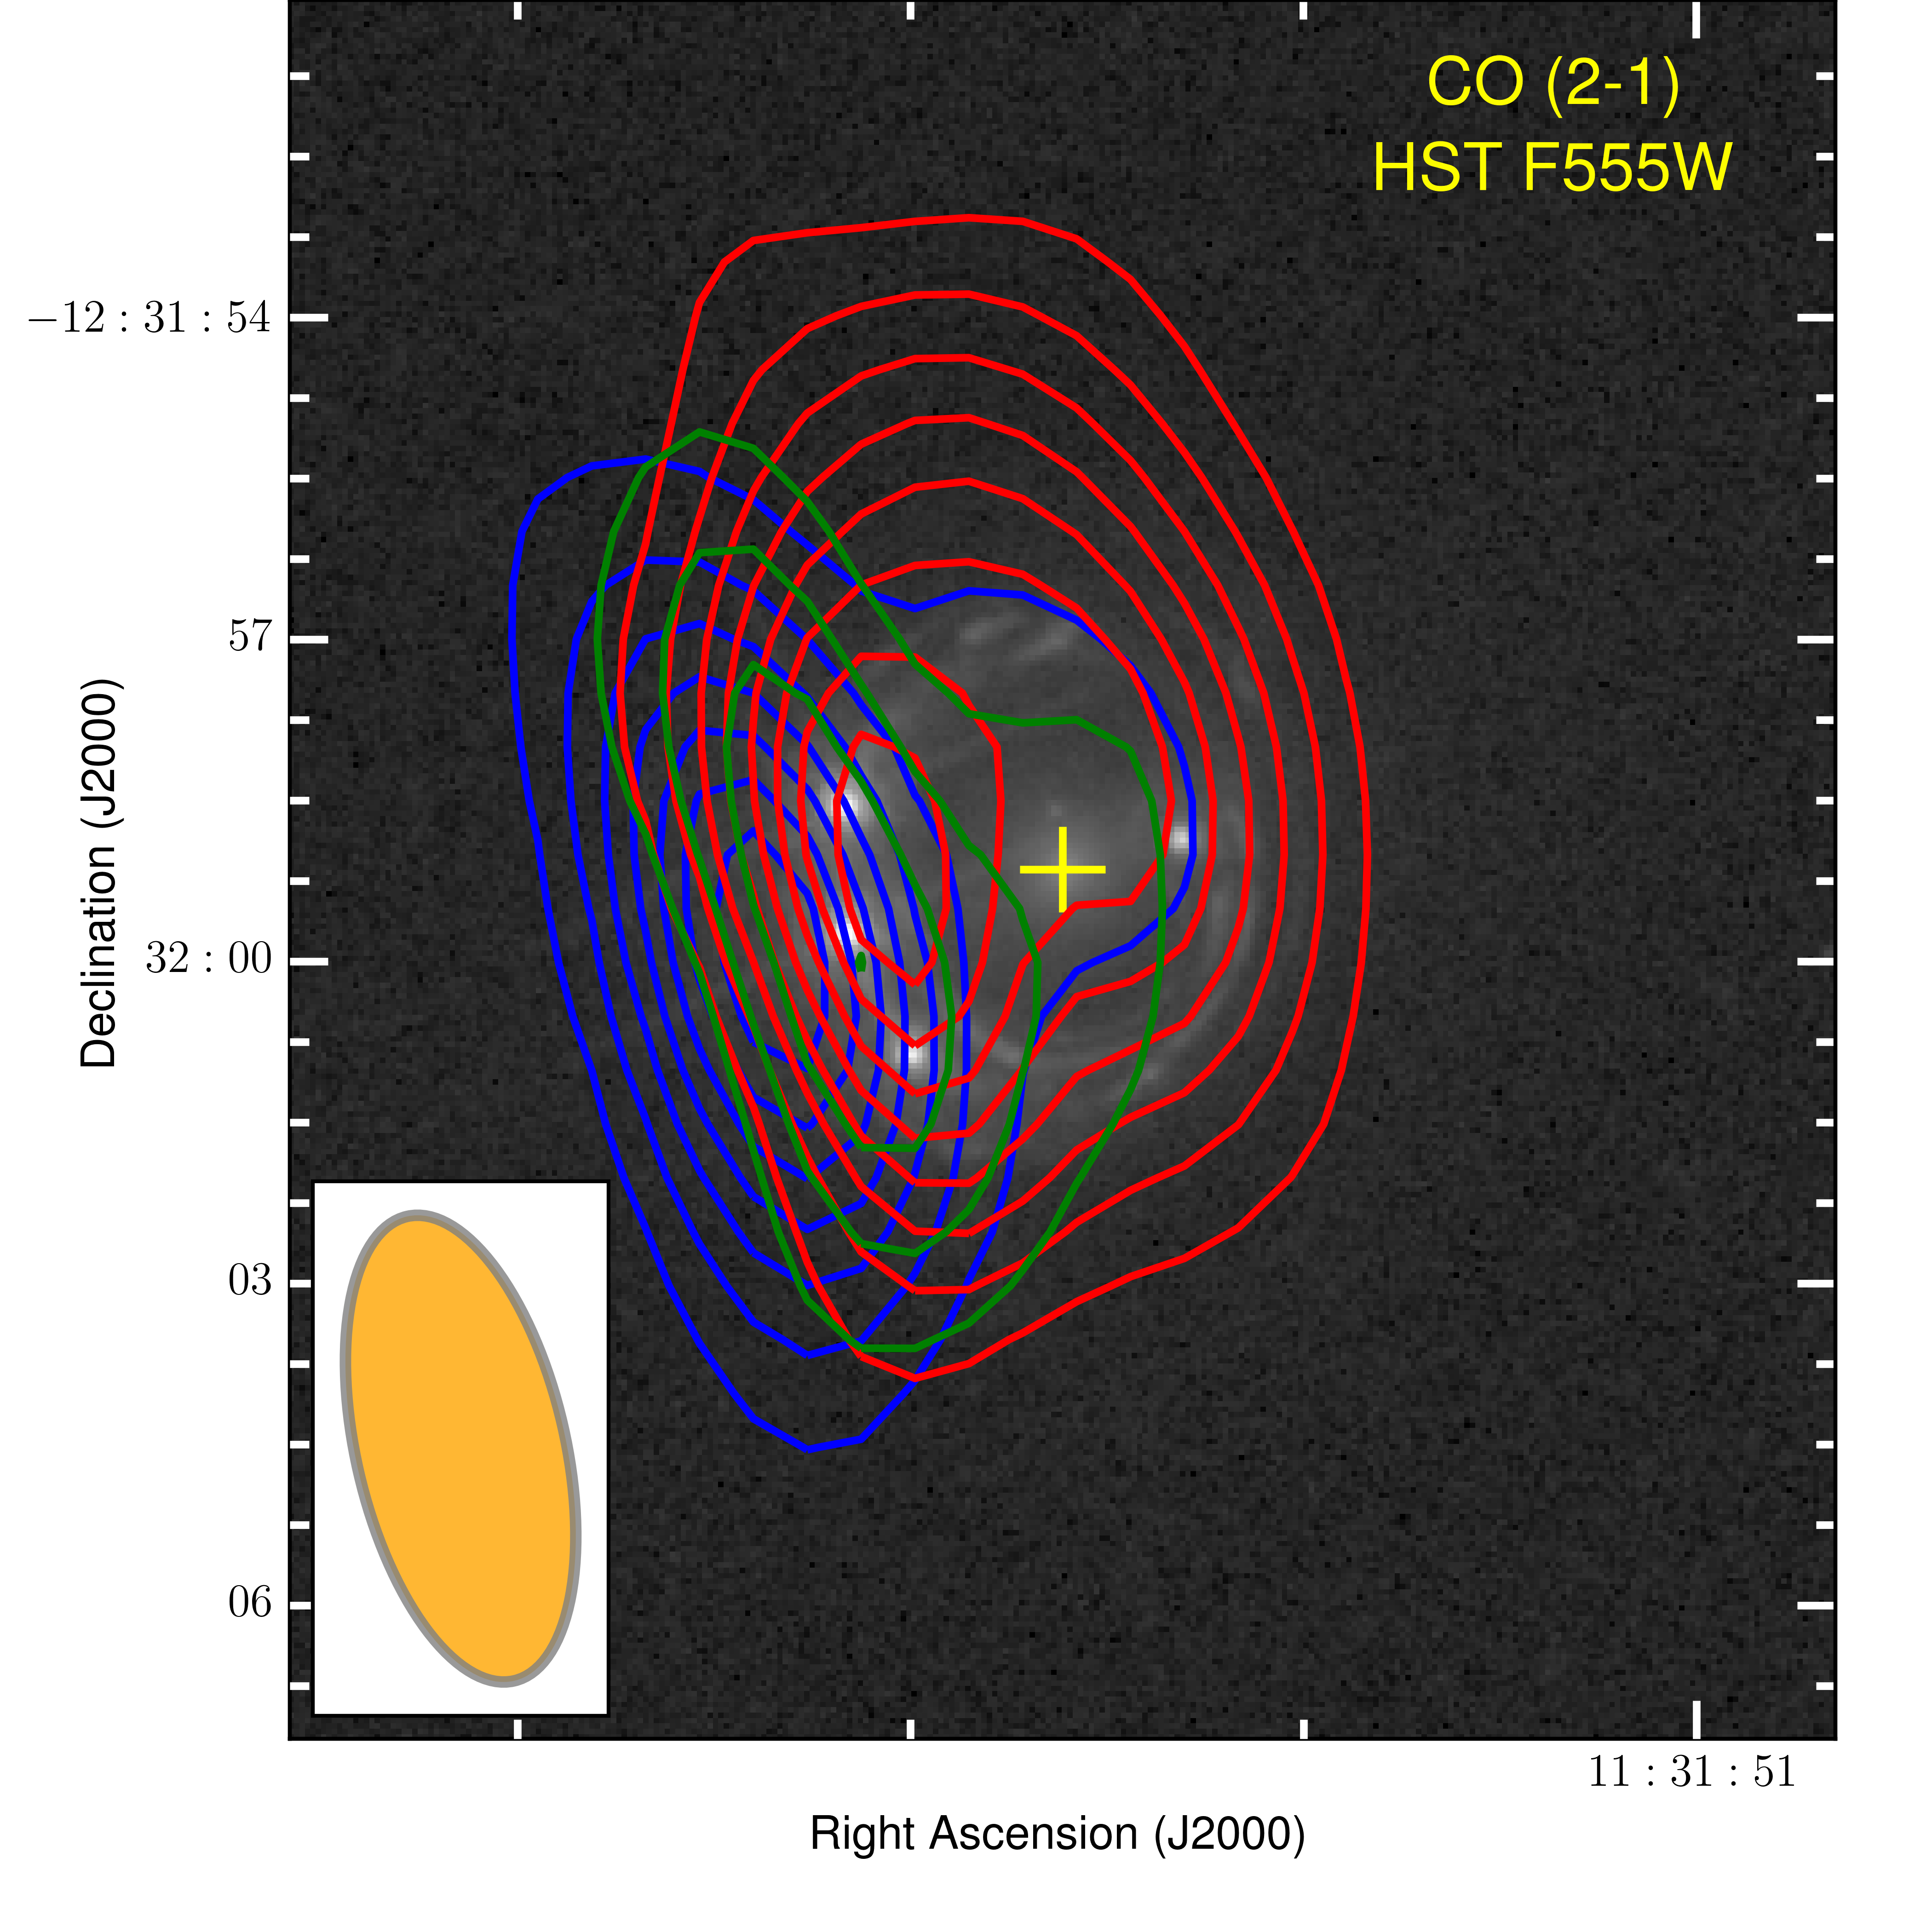
\includegraphics[width=0.35\textwidth]{../Figures/F555W_REDCentBLUE.png}
\includegraphics[width=0.55\textwidth]{../Figures/SpecCO21_twinx.eps}
\caption{
0th Moment map of CO(2-1) emission on HST F555W. moment-0: no clipping, of $\sigma$ 0.43 mJy beam\pmOne. 
Spectrum. Velocity scale w.r.t z=0.655
 \label{fig:CO21mom0}}
\end{figure*}


\begin{figure}[tbph]
\centering
\includegraphics[width=0.5\textwidth]{../Figures/CO_highOmom_CLIP5sigma}       
\caption{
1st and 2nd order moments, clipped at 5 $\sigma$. 1st moment contour steps of 50 \kms, 2nd moment steps of 100 \kms.
velocity range in z=0 frame = [-530.33, 72.73] \kms
chan = [127, 155] 
sigma = 0.16821825 Jy \kms per Beam
theshold: 5*sigma = 7.2550e-3 Jy per beam (per channel)
 \label{fig:highOmoments}}
\end{figure}




\begin{figure*}[tbph]
\centering
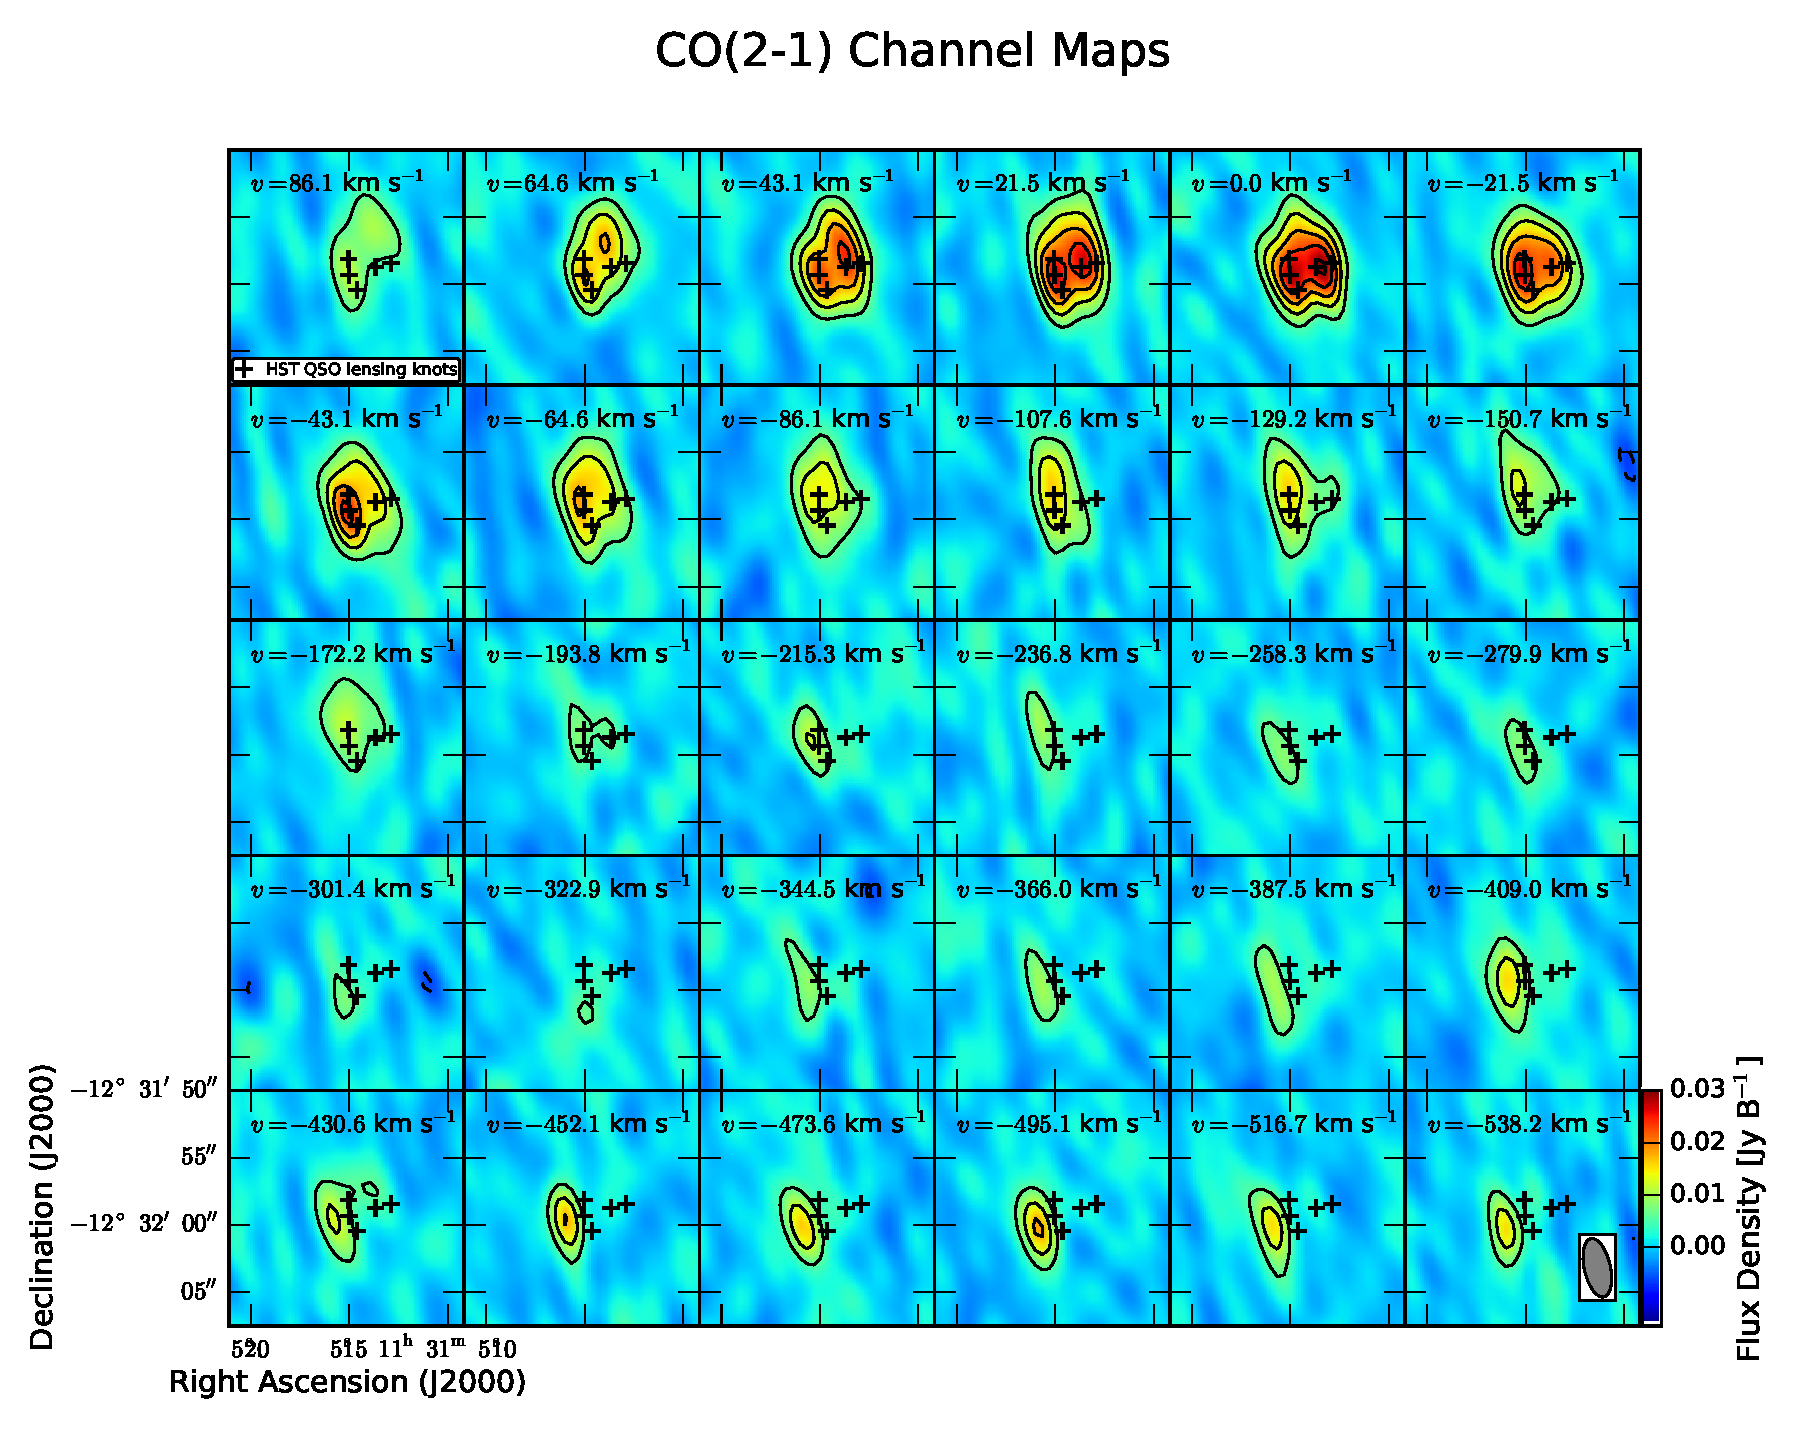
\includegraphics[width=\textwidth]{../Figures/co_channel_maps.eps}	 %
\caption{
Black crosses indicate the position of the lensed AGN (components ABCD) and the central white-filled star indicates the
position of the foreground lensing galaxy (component G) as detected in the HST image.
 \label{fig:chanmap}}
\end{figure*}

\begin{figure*}[tbph]
\centering
\includegraphics[width=\textwidth]{../Figures/spatialSpec_offsetShifted.eps}   
\caption{ 
Spatial spectra, binned by 3 pixels in each direction (1\farcs5)
 \label{fig:spatialSpec}}
\end{figure*}



\section{Continuum}

% 2mm continuum averaged over chan 1 120 165 360
% number of channels = 316
% sigma = 1.451 mJy/B / sqrt(316) = 0.081625 mJy/B 
% go noise on map (whole map) after cleaning: 89.274 �Jy/B
% F = 1.2 mJy (integrated spatially, from ~ 1 sigma contour; 150 pixels)


\begin{figure*}[tbph]
\centering
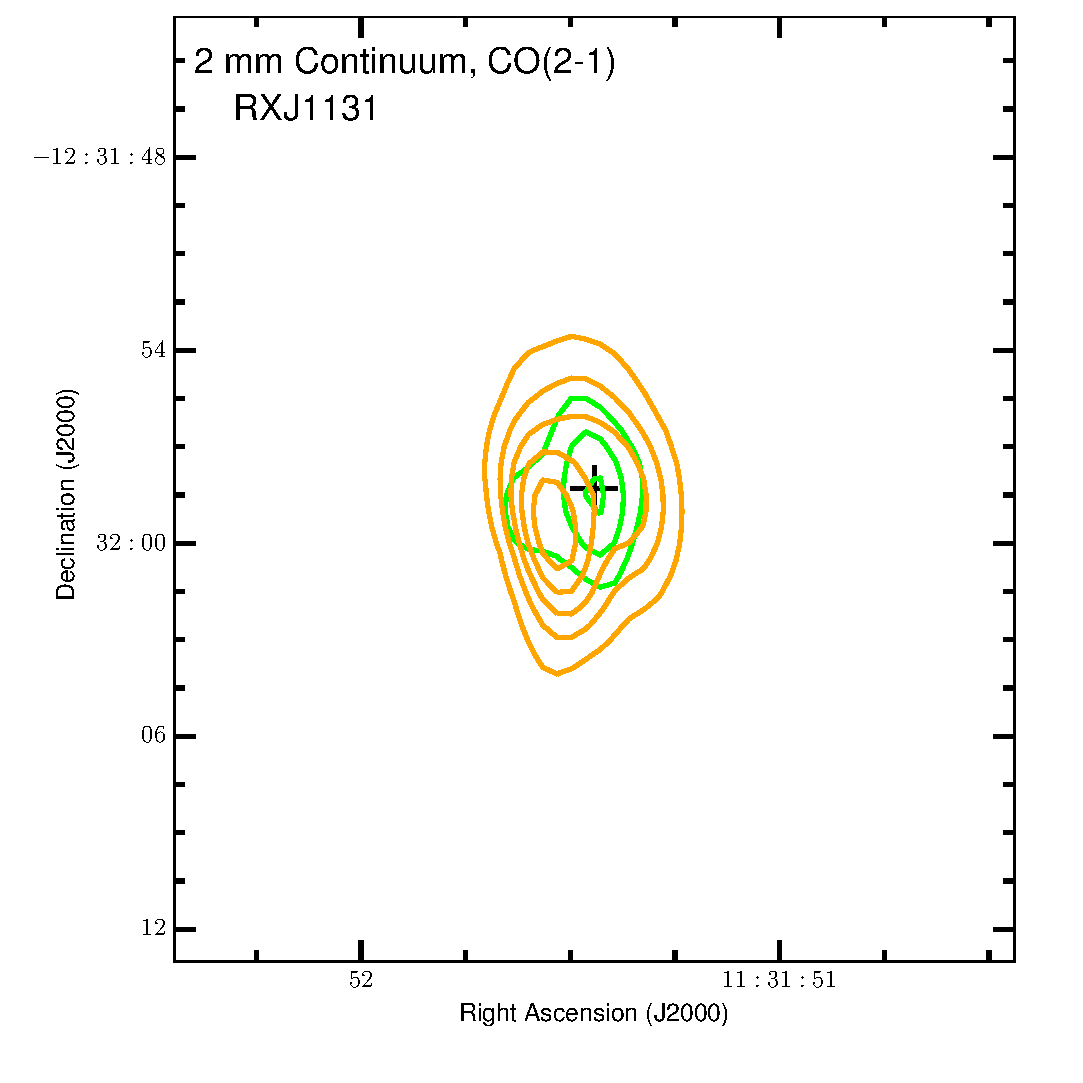
\includegraphics[width=0.8\textwidth]{../Figures/ContCO21.eps}	  
\caption{CO 21 moment0 with coninuum
 \label{fig:}}
\end{figure*}

\begin{figure*}[tbph]
\centering
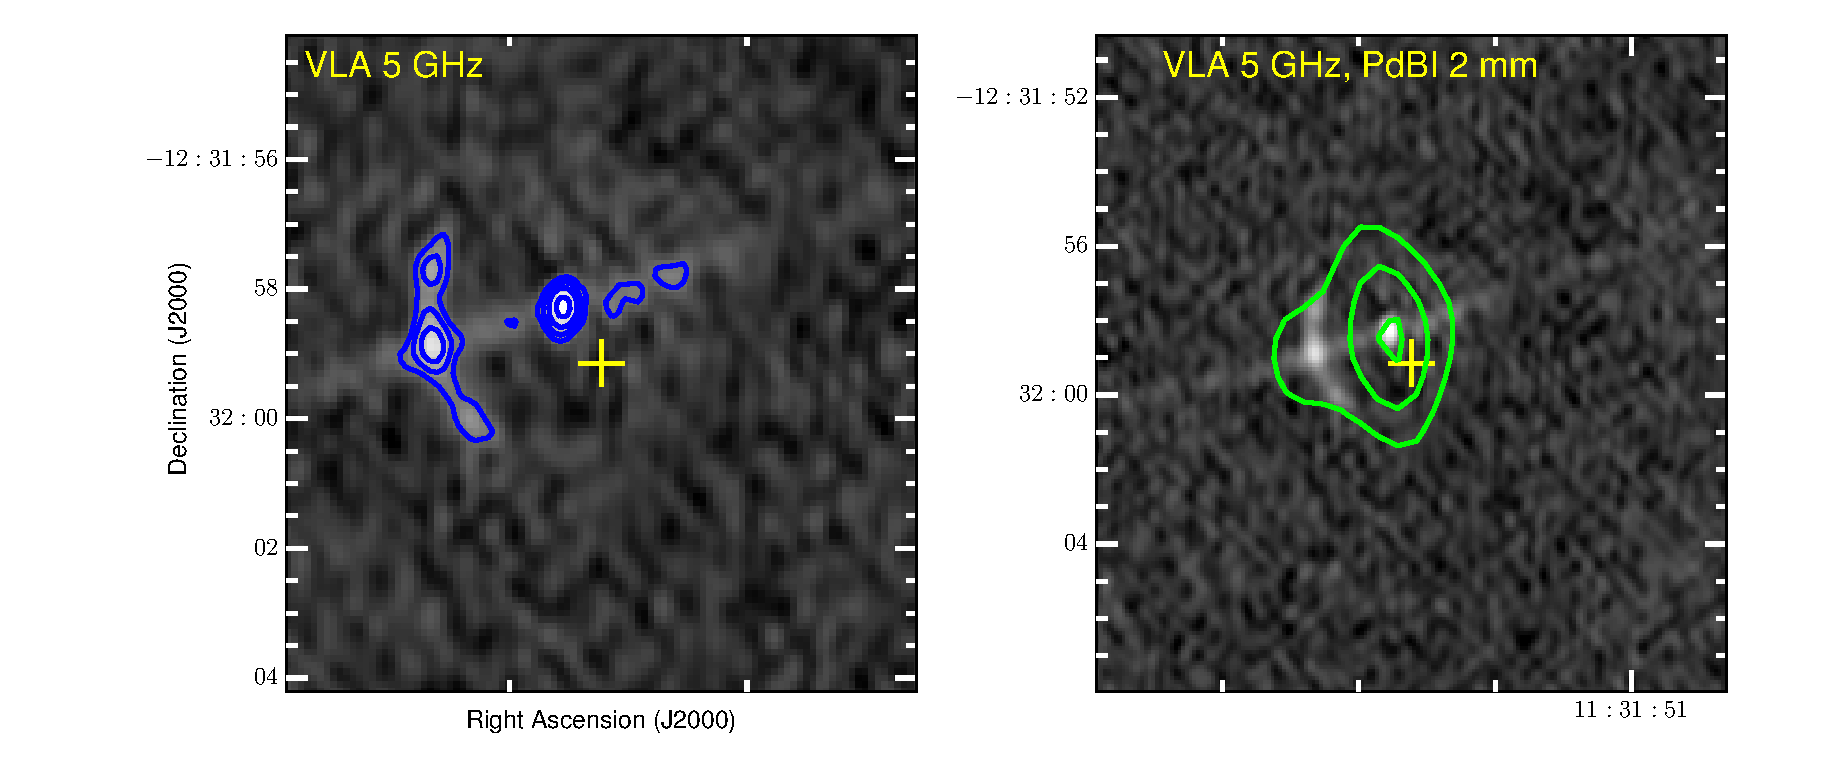
\includegraphics[width=0.8\textwidth]{../Figures/Cont2mm_5GHz_double.eps}    
\caption{VLA 5GHz continuum and PdBI 2mm continuum
 \label{fig:}}
\end{figure*}


\begin{figure*}[tbph]
\centering
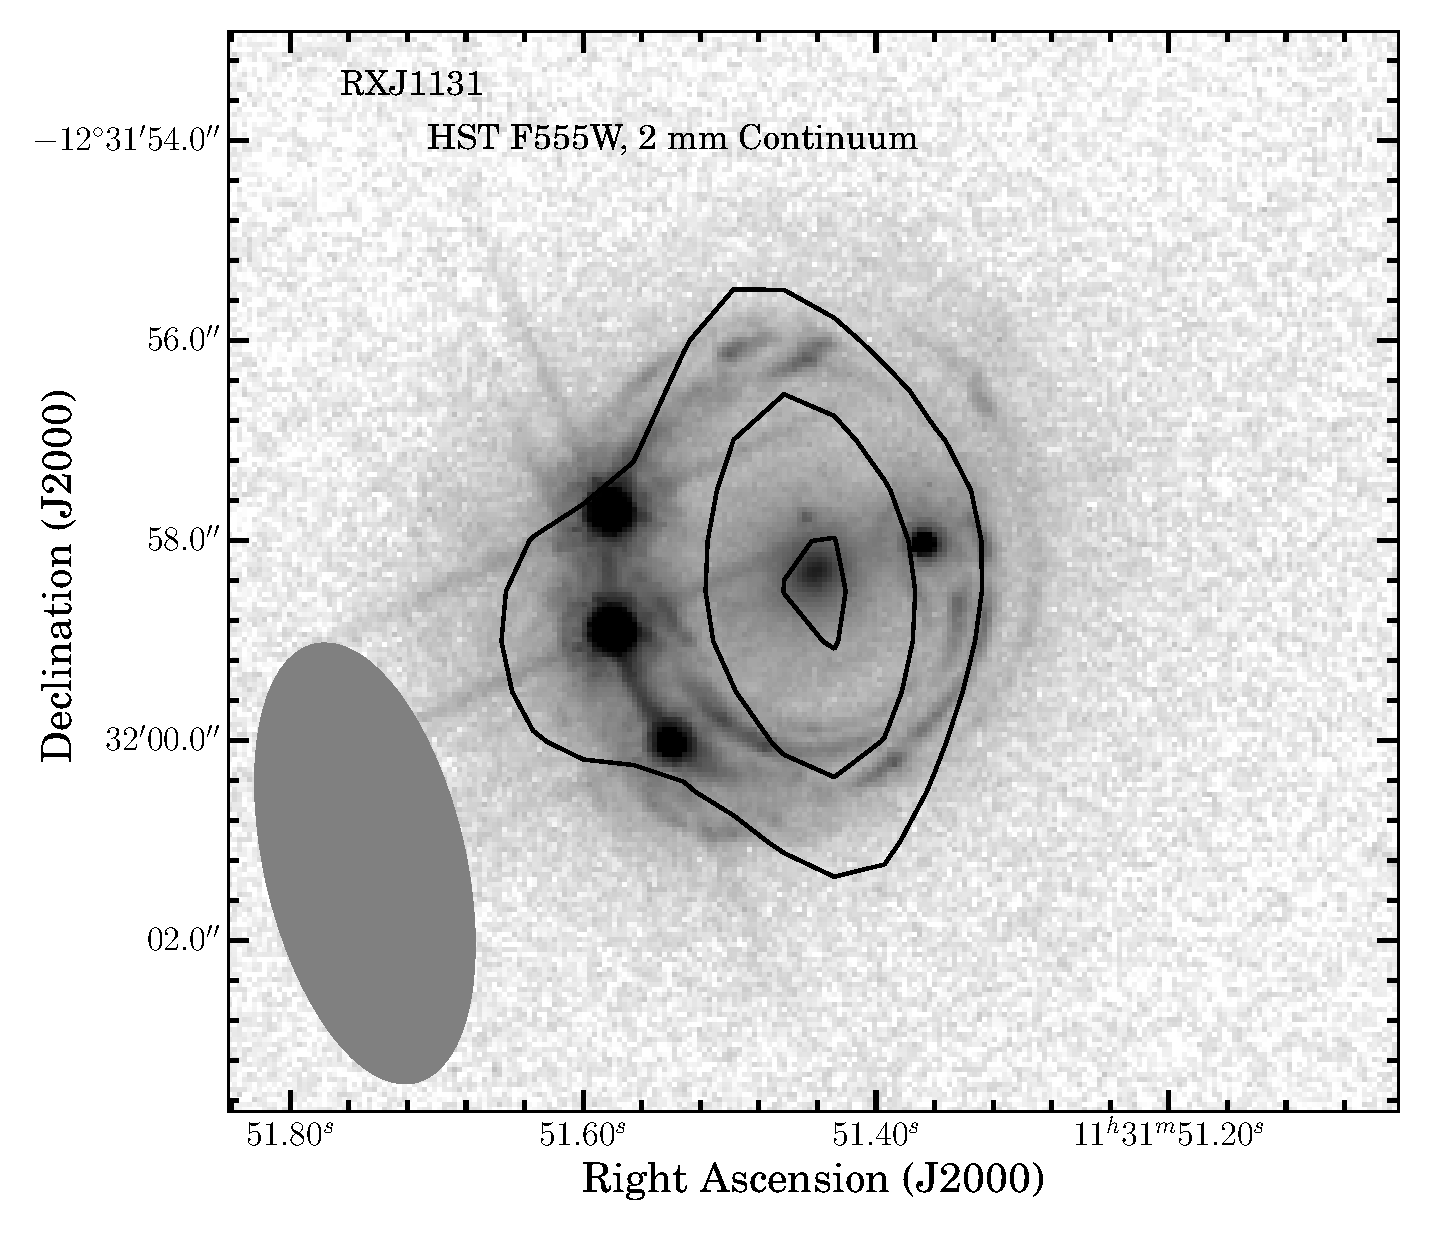
\includegraphics[width=0.35\textwidth]{../Figures/F555W_ContPdBI.eps}
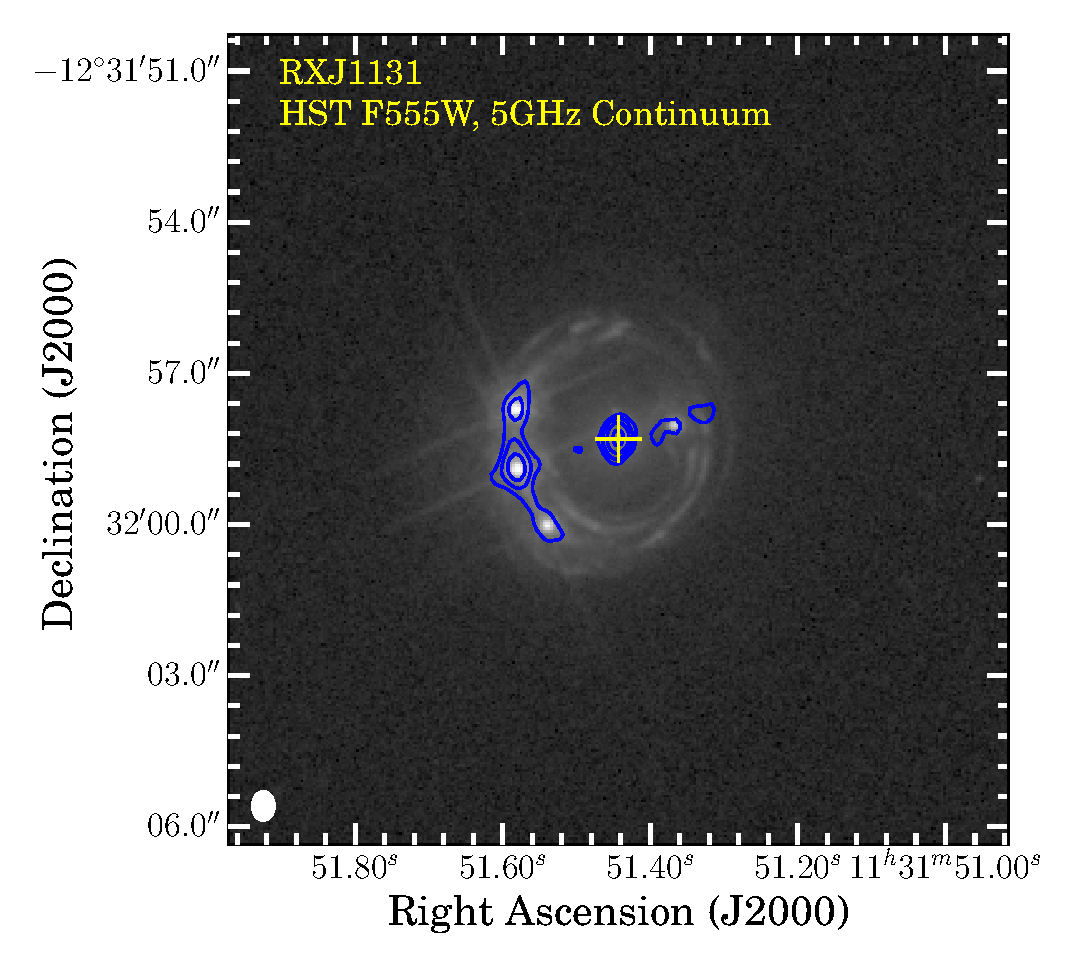
\includegraphics[width=0.55\textwidth]{../Figures/F555W_ContVLA.eps}
\caption{
can kill left figure eventually by combining this to ContCO21.eps
Right: alignment of HST and VLA 5 GHz continuum
 \label{fig:}}
\end{figure*}


%%%%%%%%%%%%%%%%%%%%%%%%%%%%%%%%%%%%%%%%%%
\section{SED}

We fit SED models to the photometry of dust emission in RXJ1131-1231 with a power-law attached to the blue side and including the 24.0\micron data from Spitzer/MIPS to constrain the dust peak.


\begin{figure*}[tbph]
\centering
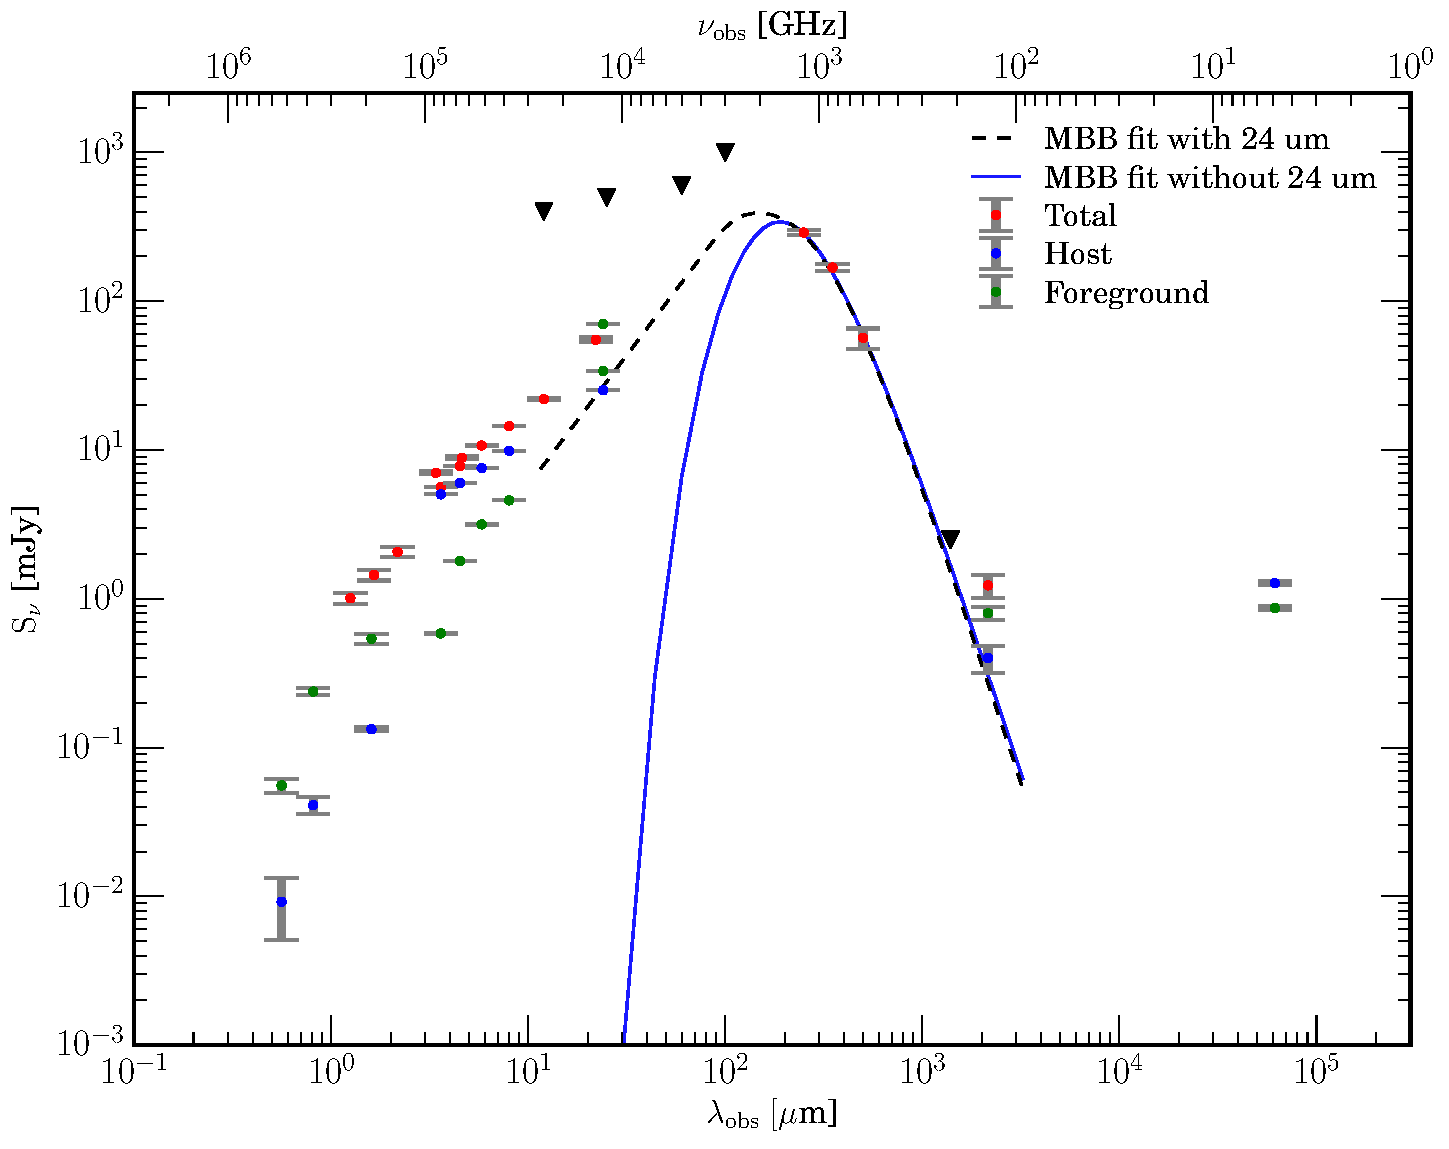
\includegraphics[width=0.8\textwidth]{../Figures/FullSED.eps}	 
\caption{VLA 5GHz continuum and PdBI 2mm continuum
TODO: change sym indicating the VLA data, (now two points at the same frequency), change sym for the 2 points on 2mm PdBI (now integrated and peak), might want to extract flux after removing a point source model.
Note THAT the WISE flux is higher than the IRAC data, probably just due to the smaller aperture used in Spitzer flux extraction, which might not be resolving the source and not including everything. 
Might want to add NVSS constraints.
 \label{fig:}}
\end{figure*}

\begin{deluxetable}{lccc}[tbpH]
\tabletypesize{\scriptsize}
\tablecolumns{4}
\tablecaption{Photometry data}
\tablehead{\colhead{Wavelength } & \colhead{Frequency } & \colhead{Flux Density } & \colhead{Instrument}\\ \colhead{micron} & \colhead{GHz} & \colhead{mJy} & \colhead{ }}
\startdata
0.555 & 540167.0 & 0.056 $\pm$ 0.006 & HST-ACS/V-Band(L) \\
0.555 & 540167.0 & 0.009 $\pm$ 0.0041 & HST-ACS/V-Band(H) \\
0.814 & 368295.0 & 0.238 $\pm$ 0.013 & HST-ACS/I-Band(L) \\
0.814 & 368295.0 & 0.041 $\pm$ 0.0054 & HST-ACS/I-Band(H) \\
1.25 & 239834.0 & 1.009 $\pm$ 0.09 & 2MASS/J-Band \\
1.6 & 187370.0 & 0.539 $\pm$ 0.041 & HST-NICMOS(NIC2)/H-Band(L) \\
1.6 & 187370.0 & 0.133 $\pm$ 0.004 & HST-NICMOS(NIC2)/H-Band(H) \\
1.65 & 181692.0 & 1.448 $\pm$ 0.12 & 2MASS/H-Band \\
2.17 & 138153.0 & 2.064 $\pm$ 0.16 & 2MASS/Ks-Band \\
3.4 & 88174.2 & 7.027 $\pm$ 0.14 & WISE/W1 \\
3.6 & 83275.7 & 5.618 $\pm$ 0.0021 & Spitzer/IRAC(Extracted) \\
3.6 & 83275.7 & 5.034 $\pm$ 0.0021 & Spitzer/IRAC(Host) \\
3.6 & 83275.7 & 0.585 $\pm$ 0.003 & Spitzer/IRAC(Archive-Host) \\
4.5 & 66620.5 & 7.803 $\pm$ 0.0021 & Spitzer/IRAC(Archive) \\
4.5 & 66620.5 & 6.009 $\pm$ 0.0017 & Spitzer/IRAC(Host) \\
4.5 & 66620.5 & 1.794 $\pm$ 0.0027 & Spitzer/IRAC(Archive-Host) \\
4.6 & 65172.3 & 8.872 $\pm$ 0.16 & WISE/W2 \\
5.8 & 51688.4 & 10.720 $\pm$ 0.0051 & Spitzer/IRAC(Archive) \\
5.8 & 51688.4 & 7.557 $\pm$ 0.003 & Spitzer/IRAC(Host) \\
5.8 & 51688.4 & 3.163 $\pm$ 0.0059 & Spitzer/IRAC(Archive-Host) \\
8.0 & 37474.1 & 14.470 $\pm$ 0.0041 & Spitzer/IRAC(Archive) \\
8.0 & 37474.1 & 9.881 $\pm$ 0.0039 & Spitzer/IRAC(Host) \\
8.0 & 37474.1 & 4.589 $\pm$ 0.0057 & Spitzer/IRAC(Archive-Host) \\
12.0 & 24982.7 & 21.960 $\pm$ 0.42 & WISE/W3 \\
12.0 & 24982.7 & 400.000 $\pm$ \nodata & IRAS \\
22.0 & 13626.9 & 55.110 $\pm$ 1.9 & WISE/W4 \\
24.0 & 12491.4 & 47.180 $\pm$ 0.026 & Spitzer/MIPS \\
25.0 & 11991.7 & 500.000 $\pm$ \nodata & IRAS \\
60.0 & 4996.54 & 600.000 $\pm$ \nodata & IRAS \\
100.0 & 2997.92 & 1000.000 $\pm$ \nodata & IRAS \\
250.0 & 1199.17 & 289.427 $\pm$ 9.6 & Herschel/SPIRE \\
350.0 & 856.55 & 168.229 $\pm$ 8.6 & Herschel/SPIRE \\
500.0 & 599.585 & 56.782 $\pm$ 8.8 & Herschel/SPIRE \\
1387.93 & 216.0 & 2.492 $\pm$ \nodata & CARMA \\
2152.82 & 139.256 & 1.230 $\pm$ 0.22 & PdBI-integrated \\
2152.82 & 139.256 & 0.799 $\pm$ 0.082 & PdBI-peak \\
2152.82 & 139.256 & 0.400 $\pm$ 0.082 & PdBI-removedFG \\
61414.0 & 4.8815 & 1.273 $\pm$ 0.042 & VLA/Cband-arc \\
61414.0 & 4.8815 & 0.866 $\pm$ 0.027 & VLA/Cband-core
\enddata
\label{tab:BLAH}
\tablecomments{blah}
 %TablenotegoesBetween 
\tablerefs{blah}
\end{deluxetable}






%%%%%%%%%%%%%%%
\end{document}